\documentclass[10pt]{article}
\usepackage[a4paper,margin=18mm]{geometry}
\usepackage{amsmath,amssymb,booktabs,array,enumitem,longtable}
\usepackage[T1]{fontenc}\usepackage{lmodern}
\usepackage{tikz}\usetikzlibrary{shapes.gates.logic.US,positioning,arrows.meta,patterns,calc}
\usepackage[hidelinks]{hyperref}
\setlength{\parindent}{0pt}\setlength{\parskip}{4pt}\setlength{\emergencystretch}{2em}
\newcommand{\VDD}{V_{DD}}
\newcommand{\mos}[4]{\begin{scope}[shift={(#1,#2)}]
\draw (0,.24)--(0,-.24);\draw (0,.20)--(.25,.20)--(.25,.5);
\draw (0,-.20)--(.25,-.20)--(.25,-.5);\draw (-.16,.23)--(-.16,-.23);
\ifnum#4=1\draw (-.26,0) circle (.06);\draw (-.75,0)--(-.32,0);\else\draw (-.75,0)--(-.16,0);\fi
\node[anchor=east,font=\scriptsize] at (-.76,0) {$#3$};\end{scope}}
\newcommand{\ground}[2]{\draw (#1,#2)--(#1,{#2-.12});\draw ({#1-.17},{#2-.12})--({#1+.17},{#2-.12});\draw ({#1-.11},{#2-.20})--({#1+.11},{#2-.20});}
\newcommand{\rail}[3]{\draw (#1,#2)--(#1,{#2+.14});\node[above,font=\scriptsize] at (#1,{#2+.14}) {$#3$};}
\newcommand{\hmos}[4]{\begin{scope}[shift={(#1,#2)}]
\draw(-.24,0)--(.24,0);\draw(-.2,0)--(-.2,-.25)--(-.5,-.25);\draw(.2,0)--(.2,-.25)--(.5,-.25);
\draw(-.23,.16)--(.23,.16);
\ifnum#4=1\draw(0,.26)circle(.06);\draw(0,.32)--(0,.75);\else\draw(0,.16)--(0,.75);\fi
\node[below,font=\scriptsize]at(0,-.32){#3};\end{scope}}
\newcommand{\qheading}[1]{\par\medskip\textbf{#1}\par}
\begin{document}
\begin{center}{\Large\bfseries Spring 2008 Midterm---Independent Solutions}\\EE332 Introduction to VLSI\end{center}
The complete original has two pages and five questions. It is extracted from the first two pages of a 36-page mixed-year compilation and cross-checked against two native photographs. The reconstruction includes only this paper's questions; handwritten annotations are excluded from the editable text. Q5's printed 10\% is treated as the remaining ten points of a 100-point exam.
The four matching graded booklet pages occur in reverse order on compilation pages 3--6. Their overall score is provenance, not a correctness guarantee. Identity pages remain local. Independent MOS/Boolean, delay, integer-optimization and sizing evidence is reproducible with \texttt{verify\_logic\_timing.py}; no process measurements are claimed.
\qheading{1. Concepts and static CMOS (40 points)}
\begin{enumerate}[label=(\alph*),leftmargin=7mm]
\item A conductor attached to a gate can collect charge during plasma processing and stress/damage thin gate oxide. Antenna rules limit the relevant conductor-to-gate ratio or provide a discharge path. This is a fabrication charging effect; see Li's \href{https://www.ee.ncu.edu.tw/jfli/public_html/VLSI/lecture/ch03.pdf}{Chapter 3 lecture}, slide 37.
\item In saturation, increasing drain voltage moves the pinch-off boundary toward the source and reduces effective channel length. Drain current therefore still increases with $V_{DS}$: a simple approximation is $I_D\simeq\frac12\beta(V_{GS}-V_t)^2(1+\lambda V_{DS})$. Saturation has finite output conductance; it is not the same as a perfectly constant current source.
\item The nMOS PDN is a two-device $xy$ branch in parallel with $w$ in series with parallel $u,v$. Its five-device pMOS dual is $(x\parallel y)$ in series with $[w\parallel(u\text{ series }v)]$. The complete ten-MOS schematic is on the following page; it generates the requested complemented function directly.
\item Four ideal static-CMOS properties: full rail logic levels; negligible DC supply current for stable valid inputs apart from leakage; high input resistance with mainly capacitive input loading; and a topology-determined (nonratioed) Boolean function with complementary PUN/PDN operation. Transitions can still draw short-circuit and switching current.
\item Guard rings plus frequent well/substrate taps collect injected charge and reduce parasitic well/substrate voltage drops. Isolation such as SOI interrupts the bulk parasitic PNPN path. Both reduce latchup susceptibility; an arbitrary logic transistor resize alone is not a general cure.
\item Both transistor drains join the output; the pMOS source is at $V_{DD}$ and the nMOS source at $V_{SS}$. Both gates join the input, as labeled below.
\item $NM_L=V_{IL}-V_{OL}$ and $NM_H=V_{OH}-V_{IH}$. $V_{IL},V_{IH}$ occur at the two slope-$-1$ points of the VTC. The output bounds are $V_{OL},V_{OH}$.
\item Increase separation/reduce parallel coupling length, and insert an appropriately connected supply/ground shield. Buffering and twisting have application-specific timing/symmetry requirements; these two direct approaches reduce mutual coupling.
\item Fanout gate capacitance, output diffusion/junction capacitance, and interconnect capacitance, including relevant coupling.
\end{enumerate}
\begin{center}\begin{tikzpicture}[x=.8cm,y=.8cm,font=\scriptsize]
\draw[->](0,0)--(5,0)node[right]{$V_{in}$};\draw[->](0,0)--(0,4)node[above]{$V_{out}$};
\draw plot[smooth]coordinates{(0,3.5)(1,3.4)(1.6,3.1)(2.1,2.6)(2.5,1.7)(2.9,.8)(3.4,.35)(4.5,.25)};
\draw[dashed](0,3.1)--(1.6,3.1)--(1.6,0);\draw[dashed](0,.8)--(2.9,.8)--(2.9,0);\node[left]at(0,3.1){$V_{OH}$};\node[left]at(0,.8){$V_{OL}$};\node[below]at(1.6,0){$V_{IL}$};\node[below]at(2.9,0){$V_{IH}$};
\end{tikzpicture}\quad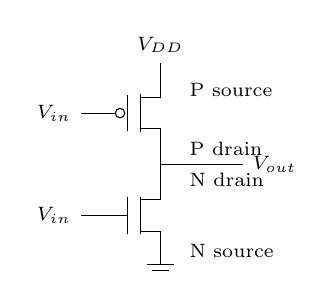
\begin{tikzpicture}[x=1cm,y=1cm,font=\scriptsize]
\mos{0}{1.5}{V_{in}}{1}\mos{0}{.2}{V_{in}}{0}\draw(.25,1)--(.25,.7);\draw(.25,.85)--(1.3,.85)node[right]{$V_{out}$};\rail{.25}{2}{V_{DD}}\ground{.25}{-.3}
\node[right]at(.5,1.8){P source};\node[right]at(.5,1.05){P drain};\node[right]at(.5,.65){N drain};\node[right]at(.5,-.25){N source};
\end{tikzpicture}\end{center}
\textbf{Reference comparison.} The graded booklet's antenna, modulation, complex-gate and terminal-label answers are largely consistent. Its static-CMOS response lists operating regions, and its noise-margin answer omits the VTC. The ungraded alternative supplies better property/VTC examples; its ``always inverted'' claim is too broad, and its $C_{gs}+C_{gd}+C_{gb}$ list describes input gate components rather than the three output-load categories.
\newpage
\begin{center}\begin{tikzpicture}[x=0.72cm,y=0.72cm,font=\scriptsize]
\begin{scope}[thin]\mos{0.0}{0.0}{x}{0}\end{scope}
\draw(0.25,0.5)--(0.25,0.75)node[above]{$ f $};
\draw(0.25,-0.5)--(0.25,-0.75)node[below]{$ \mathrm{QNj1} $};
\node[anchor=west]at(0.55,0.0){\texttt{QN1}};
\begin{scope}[thin]\mos{4.8}{0.0}{y}{0}\end{scope}
\draw(5.05,0.5)--(5.05,0.75)node[above]{$ \mathrm{QNj1} $};
\draw(5.05,-0.5)--(5.05,-0.75)node[below]{$ V_{SS} $};
\node[anchor=west]at(5.35,0.0){\texttt{QN2}};
\begin{scope}[thin]\mos{9.6}{0.0}{u}{0}\end{scope}
\draw(9.85,0.5)--(9.85,0.75)node[above]{$ f $};
\draw(9.85,-0.5)--(9.85,-0.75)node[below]{$ \mathrm{QNj2} $};
\node[anchor=west]at(10.15,0.0){\texttt{QN3}};
\begin{scope}[thin]\mos{14.399999999999999}{0.0}{v}{0}\end{scope}
\draw(14.649999999999999,0.5)--(14.649999999999999,0.75)node[above]{$ f $};
\draw(14.649999999999999,-0.5)--(14.649999999999999,-0.75)node[below]{$ \mathrm{QNj2} $};
\node[anchor=west]at(14.95,0.0){\texttt{QN4}};
\begin{scope}[thin]\mos{0.0}{-2.8}{w}{0}\end{scope}
\draw(0.25,-2.3)--(0.25,-2.05)node[above]{$ \mathrm{QNj2} $};
\draw(0.25,-3.3)--(0.25,-3.55)node[below]{$ V_{SS} $};
\node[anchor=west]at(0.55,-2.8){\texttt{QN5}};
\begin{scope}[thin]\mos{4.8}{-2.8}{x}{1}\end{scope}
\draw(5.05,-2.3)--(5.05,-2.05)node[above]{$ f $};
\draw(5.05,-3.3)--(5.05,-3.55)node[below]{$ \mathrm{QPj1} $};
\node[anchor=west]at(5.35,-2.8){\texttt{QP1}};
\begin{scope}[thin]\mos{9.6}{-2.8}{y}{1}\end{scope}
\draw(9.85,-2.3)--(9.85,-2.05)node[above]{$ f $};
\draw(9.85,-3.3)--(9.85,-3.55)node[below]{$ \mathrm{QPj1} $};
\node[anchor=west]at(10.15,-2.8){\texttt{QP2}};
\begin{scope}[thin]\mos{14.399999999999999}{-2.8}{u}{1}\end{scope}
\draw(14.649999999999999,-2.3)--(14.649999999999999,-2.05)node[above]{$ \mathrm{QPj1} $};
\draw(14.649999999999999,-3.3)--(14.649999999999999,-3.55)node[below]{$ \mathrm{QPj2} $};
\node[anchor=west]at(14.95,-2.8){\texttt{QP3}};
\begin{scope}[thin]\mos{0.0}{-5.6}{v}{1}\end{scope}
\draw(0.25,-5.1)--(0.25,-4.85)node[above]{$ \mathrm{QPj2} $};
\draw(0.25,-6.1)--(0.25,-6.35)node[below]{$ V_{DD} $};
\node[anchor=west]at(0.55,-5.6){\texttt{QP4}};
\begin{scope}[thin]\mos{4.8}{-5.6}{w}{1}\end{scope}
\draw(5.05,-5.1)--(5.05,-4.85)node[above]{$ \mathrm{QPj1} $};
\draw(5.05,-6.1)--(5.05,-6.35)node[below]{$ V_{DD} $};
\node[anchor=west]at(5.35,-5.6){\texttt{QP5}};
\end{tikzpicture}\end{center}
\small Q1(c): all ten devices. The nMOS network realizes $xy+(u+v)w$ and the pMOS network its complement. Identically named terminals are connected. nMOS bodies use $V_{SS}$ and pMOS bodies use $V_{DD}$.\normalsize\par
The switch checker exhausts all 32 combinations of $x,y,u,v,w$. Exactly one rail conducts at the output, with $f=\overline{xy+(u+v)w}$ in every case. No complemented primary input wires or output inverter are required.
\qheading{2. Actual fanout and delay conventions (20 points)}
\begin{center}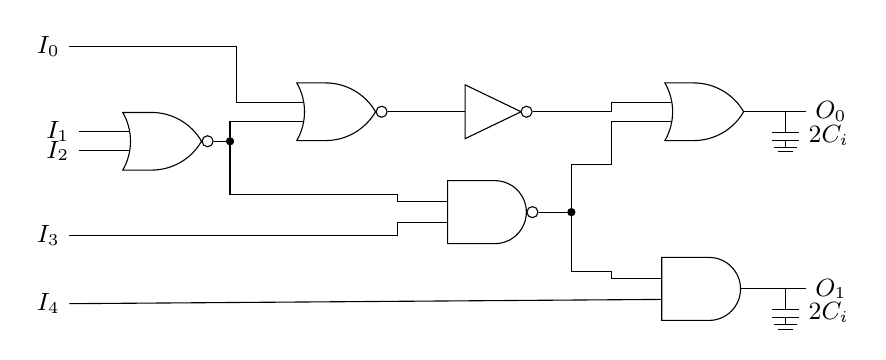
\begin{tikzpicture}[x=.85cm,y=.75cm,font=\small]
\node[nor gate US,draw,logic gate inputs=nn,minimum width=1cm](a)at(1.3,4){};
\node[nor gate US,draw,logic gate inputs=nn,minimum width=1cm](b)at(3.9,4.5){};\node[not gate US,draw,minimum width=.8cm](c)at(6.2,4.5){};
\node[or gate US,draw,logic gate inputs=nn,minimum width=1cm](o)at(9.4,4.5){};
\draw(a.input 1)--++(-.75,0)node[left]{$I_1$};\draw(a.input 2)--++(-.75,0)node[left]{$I_2$};\draw(0,5.6)node[left]{$I_0$}--(2.5,5.6)|-(b.input 1);
\draw(a.output)--(2.4,4)|-(b.input 2);\fill(2.4,4)circle(1.5pt);\draw(b.output)--(c.input);\draw(c.output)--(8.1,4.5)|-(o.input 1);
\node[nand gate US,draw,logic gate inputs=nn,minimum width=1cm](d)at(6.2,2.8){};\node[and gate US,draw,logic gate inputs=nn,minimum width=1cm](g)at(9.4,1.5){};
\draw(2.4,4)--(2.4,3.1)--(4.9,3.1)|-(d.input 1);\draw(0,2.4)node[left]{$I_3$}--(4.9,2.4)|-(d.input 2);
\draw(d.output)--(7.5,2.8)--(7.5,3.6)--(8.1,3.6)|-(o.input 2);\fill(7.5,2.8)circle(1.5pt);
\draw(7.5,2.8)--(7.5,1.8)--(8.1,1.8)|-(g.input 1);\draw(g.input 2)--(0,1.25)node[left]{$I_4$};
\foreach\gate/\y/\name in {o/4.5/0,g/1.5/1}{\draw(\gate.output)--(11,\y)node[right]{$O_\name$};\draw(10.7,\y)--(10.7,\y-.35);\draw(10.5,\y-.35)--(10.9,\y-.35);\draw(10.5,\y-.48)--(10.9,\y-.48);\ground{10.7}{\y-.48}\node[right]at(10.9,\y-.4){$2C_i$};}
\end{tikzpicture}\quad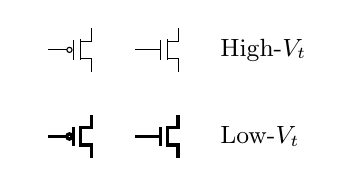
\begin{tikzpicture}[scale=.55,font=\small]
\mos{0}{3}{}{1}\mos{2}{3}{}{0}\node[right]at(3,3){High-$V_t$};
\begin{scope}[very thick]\mos{0}{1}{}{1}\mos{2}{1}{}{0}\end{scope}\node[right]at(3,1){Low-$V_t$};
\end{tikzpicture}\\\small Figure 1: (a) A CMOS circuit (b) High-/low-$V_t$ transistor symbols.\end{center}
Use $a$ for the first NOR output, $b$ for the second NOR output, $c$ for its inverted output, and $d$ for the central NAND output. The first output gate is printed \emph{OR}, and the second is \emph{AND}: apparent circles in one photograph are handwritten arcs, as confirmed directly in the independent compiled original.
\[a=\overline{I_1+I_2},\quad b=\overline{I_0+a},\quad c=\bar b=I_0+a,\quad d=\overline{aI_3}.\]
\[\boxed{O_0=c+d=1,\qquad O_1=dI_4=I_4(I_1+I_2+\bar I_3).}\]
The steady constant output does not change the requested printed gate/load network. Physical arc sums below are kept separate from whether a complete output transition can be sensitized.
\newpage
\textbf{(a) Balanced classroom mean-delay answer: $3,1.5,1,3,3.5,3.5$ units.}
The actual loads are $C_a=2C_i$ (second NOR and NAND inputs), $C_b=C_c=C_i$, and $C_d=2C_i$ (output OR and AND inputs). Both external outputs have the printed $2C_i$ load. OR/AND need an internal NOR/NAND followed by an inverter; that internal node drives $C_i$.
The following table assumes $R_p=R_n=R$ for the reference inverter, and normalizes $RC_i=1$. Series devices multiply resistance; parallel devices use the conventional worst single conducting branch for each edge. The scalar gate delay is the mean of rise and fall.
\begin{center}\begin{tabular}{lllll}\toprule Gate&Actual load&Output rise&Output fall&Mean\\\midrule
NOR$(I_1,I_2)$&$2C_i$&4&2&3\\
NOR$(I_0,a)$&$C_i$&2&1&1.5\\
INV$(b)$&$C_i$&1&1&1\\
NAND$(a,I_3)$&$2C_i$&2&4&3\\
OR$(c,d)$&internal $C_i$, output $2C_i$&$1+2=3$&$2+2=4$&3.5\\
AND$(d,I_4)$&internal $C_i$, output $2C_i$&$2+2=4$&$1+2=3$&3.5\\\bottomrule\end{tabular}\end{center}
The graded booklet's load-independent NOR/NAND 1.5 and OR 2.5 values do not include the printed fanout and $2C_i$ output loads. A direct four-device AND drawing is also incomplete: positive AND requires an output inverter. The ungraded two-page study answer independently agrees with the actual-load results 3, 1.5, 3, 3.5 and 3.5; the standalone inverter contributes the remaining 1 unit.
\textbf{General resistance ratio.} The given p/n widths 2/1 do not themselves specify the mobility or turn-on resistance ratio. If $r=R_p/R_n$ and the reference mean delay is $\tfrac12(R_p+R_n)C_i=1$, define
\[n_r=\frac{2r+1}{r+1},\qquad a_r=\frac{r+2}{r+1}.\]
The six mean gate delays in table order are
\[\boxed{2n_r,\quad n_r,\quad1,\quad2a_r,\quad n_r+2,\quad a_r+2.}\]
The balanced example follows at $r=1$, requiring approximately $\mu_n/\mu_p=2$ with the printed geometry and matched threshold magnitudes. That process ratio is not printed in Q2, so the general result is retained rather than presented as an unconditional numerical derivation.
\textbf{Path sums.} Under the balanced mean-delay convention, the longest printed paths are first NOR$\to$NAND$\to$output OR/AND, each $3+3+3.5=9.5$ units. The upper first NOR$\to$second NOR$\to$INV$\to$OR path is $3+1.5+1+3.5=9$ units. The saved CSV also lists separate rise/fall arc sums. The longest sensitizable $O_1$ edge is 11 units; the conservative $O_0$ physical fall-arc sum is 12 units, but $O_0$ is steady constant 1 and that sum is not a measured or guaranteed output edge.
\newpage
\textbf{(b) A conditional 20L/6H transistor implementation.}
Keep the common first NOR, the central NAND, and both complete output gates low-$V_t$. Make the upper second NOR and its following inverter high-$V_t$ only when their available slack permits. All 26 original MOS and complete positive OR/AND inverters are shown. Thick=L; thin=H; every device is also labeled H/L.
\begin{center}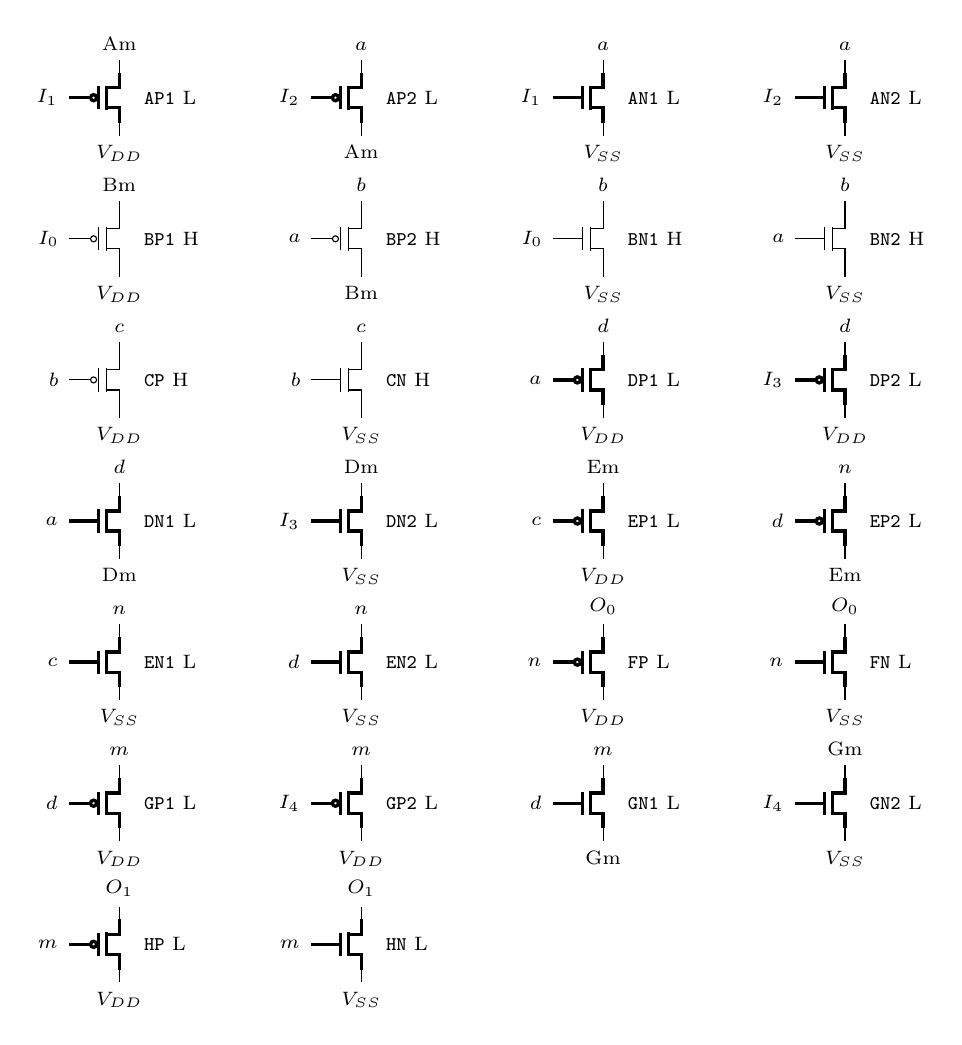
\begin{tikzpicture}[x=0.64cm,y=0.64cm,font=\scriptsize]
\begin{scope}[very thick]\mos{0.0}{0.0}{I_1}{1}\end{scope}
\draw(0.25,0.5)--(0.25,0.75)node[above]{$ \mathrm{Am} $};
\draw(0.25,-0.5)--(0.25,-0.75)node[below]{$ V_{DD} $};
\node[anchor=west]at(0.55,0.0){\texttt{AP1} L};
\begin{scope}[very thick]\mos{4.8}{0.0}{I_2}{1}\end{scope}
\draw(5.05,0.5)--(5.05,0.75)node[above]{$ a $};
\draw(5.05,-0.5)--(5.05,-0.75)node[below]{$ \mathrm{Am} $};
\node[anchor=west]at(5.35,0.0){\texttt{AP2} L};
\begin{scope}[very thick]\mos{9.6}{0.0}{I_1}{0}\end{scope}
\draw(9.85,0.5)--(9.85,0.75)node[above]{$ a $};
\draw(9.85,-0.5)--(9.85,-0.75)node[below]{$ V_{SS} $};
\node[anchor=west]at(10.15,0.0){\texttt{AN1} L};
\begin{scope}[very thick]\mos{14.399999999999999}{0.0}{I_2}{0}\end{scope}
\draw(14.649999999999999,0.5)--(14.649999999999999,0.75)node[above]{$ a $};
\draw(14.649999999999999,-0.5)--(14.649999999999999,-0.75)node[below]{$ V_{SS} $};
\node[anchor=west]at(14.95,0.0){\texttt{AN2} L};
\begin{scope}[thin]\mos{0.0}{-2.8}{I_0}{1}\end{scope}
\draw(0.25,-2.3)--(0.25,-2.05)node[above]{$ \mathrm{Bm} $};
\draw(0.25,-3.3)--(0.25,-3.55)node[below]{$ V_{DD} $};
\node[anchor=west]at(0.55,-2.8){\texttt{BP1} H};
\begin{scope}[thin]\mos{4.8}{-2.8}{a}{1}\end{scope}
\draw(5.05,-2.3)--(5.05,-2.05)node[above]{$ b $};
\draw(5.05,-3.3)--(5.05,-3.55)node[below]{$ \mathrm{Bm} $};
\node[anchor=west]at(5.35,-2.8){\texttt{BP2} H};
\begin{scope}[thin]\mos{9.6}{-2.8}{I_0}{0}\end{scope}
\draw(9.85,-2.3)--(9.85,-2.05)node[above]{$ b $};
\draw(9.85,-3.3)--(9.85,-3.55)node[below]{$ V_{SS} $};
\node[anchor=west]at(10.15,-2.8){\texttt{BN1} H};
\begin{scope}[thin]\mos{14.399999999999999}{-2.8}{a}{0}\end{scope}
\draw(14.649999999999999,-2.3)--(14.649999999999999,-2.05)node[above]{$ b $};
\draw(14.649999999999999,-3.3)--(14.649999999999999,-3.55)node[below]{$ V_{SS} $};
\node[anchor=west]at(14.95,-2.8){\texttt{BN2} H};
\begin{scope}[thin]\mos{0.0}{-5.6}{b}{1}\end{scope}
\draw(0.25,-5.1)--(0.25,-4.85)node[above]{$ c $};
\draw(0.25,-6.1)--(0.25,-6.35)node[below]{$ V_{DD} $};
\node[anchor=west]at(0.55,-5.6){\texttt{CP} H};
\begin{scope}[thin]\mos{4.8}{-5.6}{b}{0}\end{scope}
\draw(5.05,-5.1)--(5.05,-4.85)node[above]{$ c $};
\draw(5.05,-6.1)--(5.05,-6.35)node[below]{$ V_{SS} $};
\node[anchor=west]at(5.35,-5.6){\texttt{CN} H};
\begin{scope}[very thick]\mos{9.6}{-5.6}{a}{1}\end{scope}
\draw(9.85,-5.1)--(9.85,-4.85)node[above]{$ d $};
\draw(9.85,-6.1)--(9.85,-6.35)node[below]{$ V_{DD} $};
\node[anchor=west]at(10.15,-5.6){\texttt{DP1} L};
\begin{scope}[very thick]\mos{14.399999999999999}{-5.6}{I_3}{1}\end{scope}
\draw(14.649999999999999,-5.1)--(14.649999999999999,-4.85)node[above]{$ d $};
\draw(14.649999999999999,-6.1)--(14.649999999999999,-6.35)node[below]{$ V_{DD} $};
\node[anchor=west]at(14.95,-5.6){\texttt{DP2} L};
\begin{scope}[very thick]\mos{0.0}{-8.399999999999999}{a}{0}\end{scope}
\draw(0.25,-7.899999999999999)--(0.25,-7.649999999999999)node[above]{$ d $};
\draw(0.25,-8.899999999999999)--(0.25,-9.149999999999999)node[below]{$ \mathrm{Dm} $};
\node[anchor=west]at(0.55,-8.399999999999999){\texttt{DN1} L};
\begin{scope}[very thick]\mos{4.8}{-8.399999999999999}{I_3}{0}\end{scope}
\draw(5.05,-7.899999999999999)--(5.05,-7.649999999999999)node[above]{$ \mathrm{Dm} $};
\draw(5.05,-8.899999999999999)--(5.05,-9.149999999999999)node[below]{$ V_{SS} $};
\node[anchor=west]at(5.35,-8.399999999999999){\texttt{DN2} L};
\begin{scope}[very thick]\mos{9.6}{-8.399999999999999}{c}{1}\end{scope}
\draw(9.85,-7.899999999999999)--(9.85,-7.649999999999999)node[above]{$ \mathrm{Em} $};
\draw(9.85,-8.899999999999999)--(9.85,-9.149999999999999)node[below]{$ V_{DD} $};
\node[anchor=west]at(10.15,-8.399999999999999){\texttt{EP1} L};
\begin{scope}[very thick]\mos{14.399999999999999}{-8.399999999999999}{d}{1}\end{scope}
\draw(14.649999999999999,-7.899999999999999)--(14.649999999999999,-7.649999999999999)node[above]{$ n $};
\draw(14.649999999999999,-8.899999999999999)--(14.649999999999999,-9.149999999999999)node[below]{$ \mathrm{Em} $};
\node[anchor=west]at(14.95,-8.399999999999999){\texttt{EP2} L};
\begin{scope}[very thick]\mos{0.0}{-11.2}{c}{0}\end{scope}
\draw(0.25,-10.7)--(0.25,-10.45)node[above]{$ n $};
\draw(0.25,-11.7)--(0.25,-11.95)node[below]{$ V_{SS} $};
\node[anchor=west]at(0.55,-11.2){\texttt{EN1} L};
\begin{scope}[very thick]\mos{4.8}{-11.2}{d}{0}\end{scope}
\draw(5.05,-10.7)--(5.05,-10.45)node[above]{$ n $};
\draw(5.05,-11.7)--(5.05,-11.95)node[below]{$ V_{SS} $};
\node[anchor=west]at(5.35,-11.2){\texttt{EN2} L};
\begin{scope}[very thick]\mos{9.6}{-11.2}{n}{1}\end{scope}
\draw(9.85,-10.7)--(9.85,-10.45)node[above]{$ O_0 $};
\draw(9.85,-11.7)--(9.85,-11.95)node[below]{$ V_{DD} $};
\node[anchor=west]at(10.15,-11.2){\texttt{FP} L};
\begin{scope}[very thick]\mos{14.399999999999999}{-11.2}{n}{0}\end{scope}
\draw(14.649999999999999,-10.7)--(14.649999999999999,-10.45)node[above]{$ O_0 $};
\draw(14.649999999999999,-11.7)--(14.649999999999999,-11.95)node[below]{$ V_{SS} $};
\node[anchor=west]at(14.95,-11.2){\texttt{FN} L};
\begin{scope}[very thick]\mos{0.0}{-14.0}{d}{1}\end{scope}
\draw(0.25,-13.5)--(0.25,-13.25)node[above]{$ m $};
\draw(0.25,-14.5)--(0.25,-14.75)node[below]{$ V_{DD} $};
\node[anchor=west]at(0.55,-14.0){\texttt{GP1} L};
\begin{scope}[very thick]\mos{4.8}{-14.0}{I_4}{1}\end{scope}
\draw(5.05,-13.5)--(5.05,-13.25)node[above]{$ m $};
\draw(5.05,-14.5)--(5.05,-14.75)node[below]{$ V_{DD} $};
\node[anchor=west]at(5.35,-14.0){\texttt{GP2} L};
\begin{scope}[very thick]\mos{9.6}{-14.0}{d}{0}\end{scope}
\draw(9.85,-13.5)--(9.85,-13.25)node[above]{$ m $};
\draw(9.85,-14.5)--(9.85,-14.75)node[below]{$ \mathrm{Gm} $};
\node[anchor=west]at(10.15,-14.0){\texttt{GN1} L};
\begin{scope}[very thick]\mos{14.399999999999999}{-14.0}{I_4}{0}\end{scope}
\draw(14.649999999999999,-13.5)--(14.649999999999999,-13.25)node[above]{$ \mathrm{Gm} $};
\draw(14.649999999999999,-14.5)--(14.649999999999999,-14.75)node[below]{$ V_{SS} $};
\node[anchor=west]at(14.95,-14.0){\texttt{GN2} L};
\begin{scope}[very thick]\mos{0.0}{-16.799999999999997}{m}{1}\end{scope}
\draw(0.25,-16.299999999999997)--(0.25,-16.049999999999997)node[above]{$ O_1 $};
\draw(0.25,-17.299999999999997)--(0.25,-17.549999999999997)node[below]{$ V_{DD} $};
\node[anchor=west]at(0.55,-16.799999999999997){\texttt{HP} L};
\begin{scope}[very thick]\mos{4.8}{-16.799999999999997}{m}{0}\end{scope}
\draw(5.05,-16.299999999999997)--(5.05,-16.049999999999997)node[above]{$ O_1 $};
\draw(5.05,-17.299999999999997)--(5.05,-17.549999999999997)node[below]{$ V_{SS} $};
\node[anchor=west]at(5.35,-16.799999999999997){\texttt{HN} L};
\end{tikzpicture}\end{center}
\small Conditional allocation: high threshold only in B/C; the original physical network is preserved. Identically named terminals are connected. nMOS bodies use $V_{SS}$ and pMOS bodies use $V_{DD}$.\normalsize\par
\newpage
For the primary mean-delay metric, the upper branch must obey
\[d_{NOR2,H}+d_{INV,H}\le d_{NAND,L}.\]
At the balanced loads, a uniform high-$V_t$ delay scale $\rho$ would require $(1.5+1)\rho\le3$, i.e. $\rho\le6/5$. The $I_0$ shortcut has more slack and is also checked against the original bound. This is an eligibility rule: if it fails, restore the affected devices to low threshold.
The original gives no high/low threshold values, high-$V_t$ delay penalty, leakage weights or switching conditions. Thus the displayed allocation is not an unconditional proof of global minimum leakage or unchanged measured speed. More selective substitutions may exploit transistor-level slack once characterized. The student's blanket ``critical low, other high'' rule is directionally sensible but needs actual loads, output inverter completion and a delay/slack check.
An edge-based timing objective must use the rise/fall table rather than the mean bound. In the balanced isolated-$a$ model with $I_0=0,I_3=1$, $a\uparrow$ gives $c\uparrow$ after 2 units and $d\downarrow$ after 4; $a\downarrow$ gives $d\uparrow$ after 2 and $c\downarrow$ after 3. Both orders overlap high, so no $O_0$ pulse is generated by that model. Arbitrary input histories and device-dependent arc changes need their own checks; an average-delay path sum is not a waveform measurement.
The official \href{https://www.ee.ncu.edu.tw/jfli/public_html/VLSI/lecture/ch03.pdf}{course fabrication lecture}, slide 41, motivates the qualitative threshold/slack tradeoff. It supplies no numerical high-threshold penalty for this paper. All 32 input cases pass rail/Boolean verification independently of the illustrative threshold assignment.
\qheading{3. Optimal tapered chain and the printed power metric (20 points)}
\begin{center}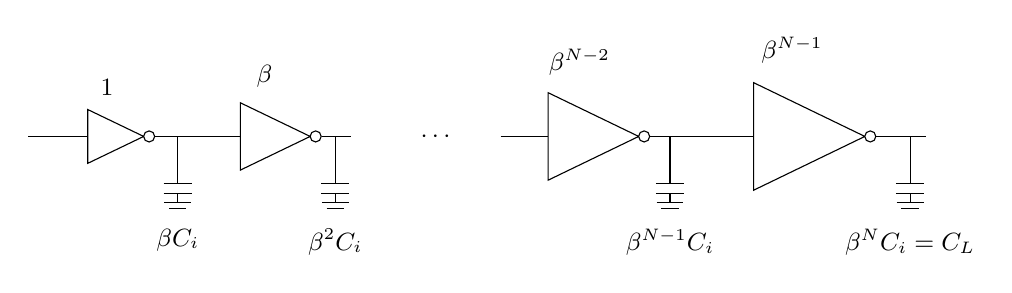
\begin{tikzpicture}[x=1cm,y=1cm,font=\small]
\node[not gate US,draw,minimum width=.8cm](a)at(0,1){};\node[not gate US,draw,minimum width=1cm](b)at(2,1){};
\node[not gate US,draw,minimum width=1.3cm](c)at(6,1){};\node[not gate US,draw,minimum width=1.6cm](d)at(8.7,1){};
\draw(-1,1)--(a.input);\draw(a.output)--(b.input);\draw(b.output)--(3.1,1);\node at(4.2,1){$\cdots$};\draw(5.0,1)--(c.input);\draw(c.output)--(d.input);\draw(d.output)--(10.4,1);
\foreach\x/\cap in {.9/\beta C_i,2.9/\beta^2C_i,7.15/\beta^{N-1}C_i,10.2/\beta^NC_i=C_L}{\draw(\x,1)--(\x,.4);\draw(\x-.18,.4)--(\x+.18,.4);\draw(\x-.18,.28)--(\x+.18,.28);\ground{\x}{.28}\node[below]at(\x,-.05){$\cap$};}
\node[above]at(0,1.4){1};\node[above]at(2,1.5){$\beta$};\node[above]at(6,1.65){$\beta^{N-2}$};\node[above]at(8.7,1.8){$\beta^{N-1}$};
\end{tikzpicture}\\\small Figure 2: A taper buffer for driving a large capacitance.\end{center}
\textbf{(a) Continuous optimum: $\beta=e$, $N=\ln(C_L/C_i)$.}
Let $F=C_L/C_i>1$ and let the first-stage resistance be $R_0$. Stage $k$ has size $\beta^{k-1}$, resistance $R_0/\beta^{k-1}$, and load $\beta^kC_i$. Every stage therefore has the same modeled delay $R_0C_i\beta$:
\[D=NR_0C_i\beta,\qquad \beta^N=F,\qquad D=R_0C_i\frac{\beta\ln F}{\ln\beta}.\]
Differentiating $\beta/\ln\beta$ gives $(\ln\beta-1)/(\ln\beta)^2=0$, hence $\beta=e$ and $N=\ln F$. This unconstrained continuous result requires $N\ge1$; for $1<F<e$ the boundary $N=1$ is appropriate.
\newpage
\textbf{Real stage count is an integer.} Minimize $D_N=R_0C_iNF^{1/N}$ for integer $N\ge1$. Since the continuous derivative changes sign at $N=\ln F$, compare $\max(1,\lfloor\ln F\rfloor)$ and $\max(1,\lceil\ln F\rceil)$ and use $\beta=F^{1/N}$. Do not round $N$ while leaving $\beta=e$ and thereby miss the required load. If noninverting polarity is required, restrict to even $N$; no such parity constraint is stated in the question.
For example, $F=64$ has continuous $N=4.159$ and integer optimum $N=4$, $\beta=64^{1/4}=2.828$. Its delay is $11.314R_0C_i$. The verifier checks seven load ratios against an explicit integer search and separately records even-stage alternatives. The matching student's continuous derivation is consistent, but an implementable integer count needs this correction.
\textbf{(b) Preserve the printed definition $\eta=(P_T-P_L)/P_T$.}
Let $K=a_{01}fV_{DD}^2C_i$ for a common stationary charging activity. With only gate loads and the final capacitance,
\[P_T=K\sum_{k=1}^N\beta^k=K\frac{\beta(\beta^N-1)}{\beta-1},\qquad P_L=K\beta^N.\]
Therefore
\[\boxed{\eta=\frac{\beta^{N-1}-1}{\beta^N-1}.}\]
It is the fraction spent on intermediate capacitances, despite the printed name ``power efficiency.'' The useful-load fraction is $1-\eta$. With the continuous optimum and $F\ge e$,
\[\eta_{cont}=\frac{F/e-1}{F-1}\quad\longrightarrow\quad\frac1e\ \text{as }F\to\infty.\]
Use the exact integer optimum's $\beta,N$ for an actual chain. For $N=1$, $\eta=0$ because only the external load is charged. Omitting the first-stage output capacitor or reversing the stated fraction changes the answer. The student's intermediate expression $1-\beta^N/\sum\beta^k$ is consistent; the exact finite-load/integer interpretation is supplied here.
\qheading{4. Equal inverter widths under $T=6RC$ (10 points)}
With minimum nMOS resistance $R$, gate capacitance $C$, width ratio $\alpha$ and the printed $\mu_n=2\mu_p$, the pMOS resistance is $2R/\alpha$ and each next inverter input is $(1+\alpha)C$. The bracket covers the first two inverters, so either input polarity sees one rise and one fall:
\[T=(R+2R/\alpha)(1+\alpha)C=RC(\alpha+3+2/\alpha).\]
Requiring $T=6RC$ gives $(\alpha-1)(\alpha-2)=0$, so $\alpha=1$ or 2. The first two output nodes have total next-stage gate load $2(1+\alpha)C$, and
\[P_{sw,1+2}=2a_{01}f(1+\alpha)CV_{DD}^2.\]
Thus $\boxed{\alpha=1}$ minimizes power subject to the delay equality. Its modeled power is $2/3$ of the $\alpha=2$ choice. The external $C_L$ after the third inverter is not in the bracketed pair; unspecified diffusion/wire loads are excluded. The student's erroneous $R_p\propto\alpha$ step is replaced by the inverse-width relation, although its corrected final $\alpha=1$ agrees.
\newpage
\qheading{5. Forward full-adder design (printed 10\%)}
The original truth table describes a forward adder taking $x,y,c_i$ and producing $s,c_o$:
\begin{center}\small Table 1: Truth table of a binary full adder.\\
\begin{tabular}{ccccc}\toprule$x$&$y$&$c_i$&$s$&$c_o$\\\midrule
0&0&0&0&0\\0&0&1&1&0\\0&1&0&1&0\\0&1&1&0&1\\
1&0&0&1&0\\1&0&1&0&1\\1&1&0&0&1\\1&1&1&1&1\\\bottomrule\end{tabular}\end{center}
\[\boxed{s=x\oplus y\oplus c_i,\qquad c_o=xy+c_i(x+y).}\]
For a complete static CMOS design, first form $\bar c_o$ from a five-nMOS PDN for $xy+c_i(x+y)$ and its five-pMOS dual, then invert to obtain $c_o$. The identity
\[s=\bar c_o(x+y+c_i)+xyc_i\]
uses only true primary inputs and that internally generated complemented carry. A seven-nMOS PDN and its seven-pMOS dual form $\bar s$, followed by the sum inverter. Total count: $(5+5+2)+(7+7+2)=28$ MOS.
The graded booklet's Q5 response treats $c_i,s,c_o$ as inputs and attempts to recover operands $x,y$, solving a different relation. The ungraded study sheet correctly gives forward-adder Boolean equations and a logic-gate diagram, but does not expand it into the required MOS schematic; the complete implementation below supplies that. The compiled original clearly shows $111\mapsto s=1,c_o=1$; the circle around the photo entry is study ink, not a changed Boolean premise.
\newpage
\begin{center}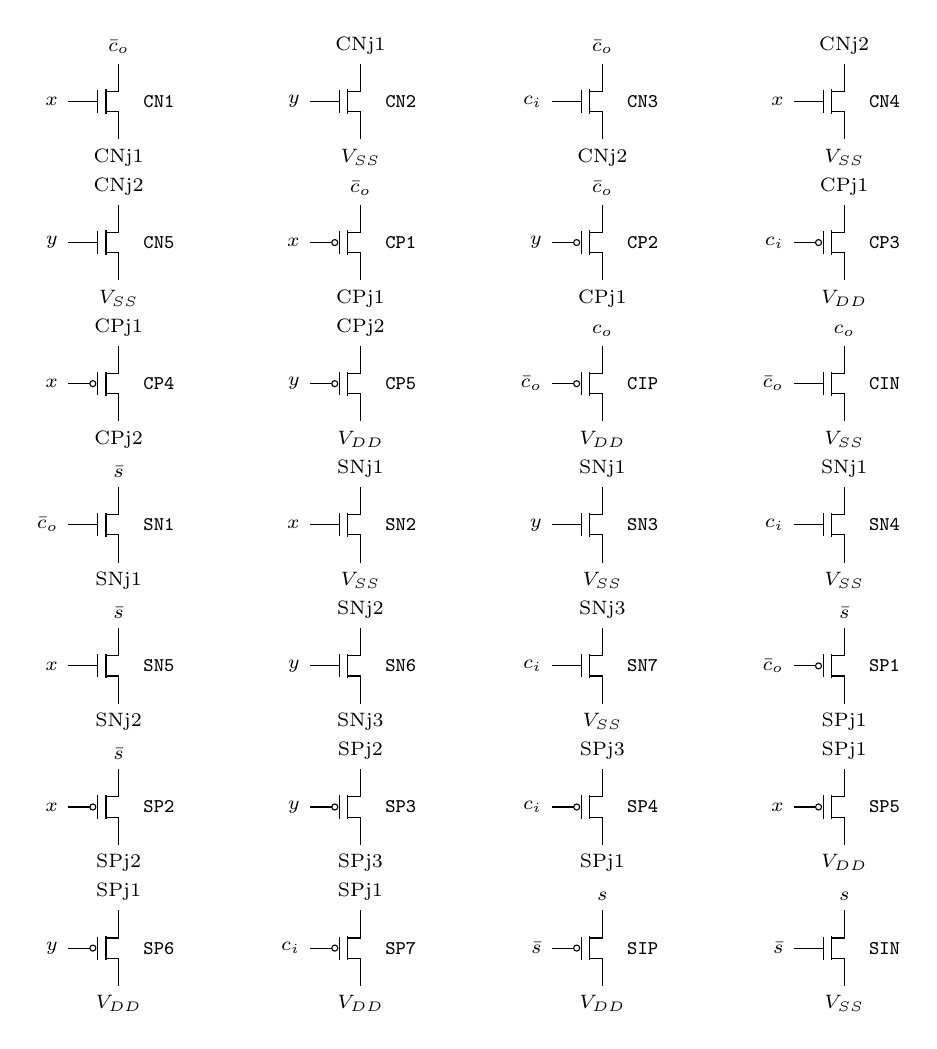
\begin{tikzpicture}[x=0.64cm,y=0.64cm,font=\scriptsize]
\begin{scope}[thin]\mos{0.0}{0.0}{x}{0}\end{scope}
\draw(0.25,0.5)--(0.25,0.75)node[above]{$ \bar c_o $};
\draw(0.25,-0.5)--(0.25,-0.75)node[below]{$ \mathrm{CNj1} $};
\node[anchor=west]at(0.55,0.0){\texttt{CN1}};
\begin{scope}[thin]\mos{4.8}{0.0}{y}{0}\end{scope}
\draw(5.05,0.5)--(5.05,0.75)node[above]{$ \mathrm{CNj1} $};
\draw(5.05,-0.5)--(5.05,-0.75)node[below]{$ V_{SS} $};
\node[anchor=west]at(5.35,0.0){\texttt{CN2}};
\begin{scope}[thin]\mos{9.6}{0.0}{c_i}{0}\end{scope}
\draw(9.85,0.5)--(9.85,0.75)node[above]{$ \bar c_o $};
\draw(9.85,-0.5)--(9.85,-0.75)node[below]{$ \mathrm{CNj2} $};
\node[anchor=west]at(10.15,0.0){\texttt{CN3}};
\begin{scope}[thin]\mos{14.399999999999999}{0.0}{x}{0}\end{scope}
\draw(14.649999999999999,0.5)--(14.649999999999999,0.75)node[above]{$ \mathrm{CNj2} $};
\draw(14.649999999999999,-0.5)--(14.649999999999999,-0.75)node[below]{$ V_{SS} $};
\node[anchor=west]at(14.95,0.0){\texttt{CN4}};
\begin{scope}[thin]\mos{0.0}{-2.8}{y}{0}\end{scope}
\draw(0.25,-2.3)--(0.25,-2.05)node[above]{$ \mathrm{CNj2} $};
\draw(0.25,-3.3)--(0.25,-3.55)node[below]{$ V_{SS} $};
\node[anchor=west]at(0.55,-2.8){\texttt{CN5}};
\begin{scope}[thin]\mos{4.8}{-2.8}{x}{1}\end{scope}
\draw(5.05,-2.3)--(5.05,-2.05)node[above]{$ \bar c_o $};
\draw(5.05,-3.3)--(5.05,-3.55)node[below]{$ \mathrm{CPj1} $};
\node[anchor=west]at(5.35,-2.8){\texttt{CP1}};
\begin{scope}[thin]\mos{9.6}{-2.8}{y}{1}\end{scope}
\draw(9.85,-2.3)--(9.85,-2.05)node[above]{$ \bar c_o $};
\draw(9.85,-3.3)--(9.85,-3.55)node[below]{$ \mathrm{CPj1} $};
\node[anchor=west]at(10.15,-2.8){\texttt{CP2}};
\begin{scope}[thin]\mos{14.399999999999999}{-2.8}{c_i}{1}\end{scope}
\draw(14.649999999999999,-2.3)--(14.649999999999999,-2.05)node[above]{$ \mathrm{CPj1} $};
\draw(14.649999999999999,-3.3)--(14.649999999999999,-3.55)node[below]{$ V_{DD} $};
\node[anchor=west]at(14.95,-2.8){\texttt{CP3}};
\begin{scope}[thin]\mos{0.0}{-5.6}{x}{1}\end{scope}
\draw(0.25,-5.1)--(0.25,-4.85)node[above]{$ \mathrm{CPj1} $};
\draw(0.25,-6.1)--(0.25,-6.35)node[below]{$ \mathrm{CPj2} $};
\node[anchor=west]at(0.55,-5.6){\texttt{CP4}};
\begin{scope}[thin]\mos{4.8}{-5.6}{y}{1}\end{scope}
\draw(5.05,-5.1)--(5.05,-4.85)node[above]{$ \mathrm{CPj2} $};
\draw(5.05,-6.1)--(5.05,-6.35)node[below]{$ V_{DD} $};
\node[anchor=west]at(5.35,-5.6){\texttt{CP5}};
\begin{scope}[thin]\mos{9.6}{-5.6}{\bar c_o}{1}\end{scope}
\draw(9.85,-5.1)--(9.85,-4.85)node[above]{$ c_o $};
\draw(9.85,-6.1)--(9.85,-6.35)node[below]{$ V_{DD} $};
\node[anchor=west]at(10.15,-5.6){\texttt{CIP}};
\begin{scope}[thin]\mos{14.399999999999999}{-5.6}{\bar c_o}{0}\end{scope}
\draw(14.649999999999999,-5.1)--(14.649999999999999,-4.85)node[above]{$ c_o $};
\draw(14.649999999999999,-6.1)--(14.649999999999999,-6.35)node[below]{$ V_{SS} $};
\node[anchor=west]at(14.95,-5.6){\texttt{CIN}};
\begin{scope}[thin]\mos{0.0}{-8.399999999999999}{\bar c_o}{0}\end{scope}
\draw(0.25,-7.899999999999999)--(0.25,-7.649999999999999)node[above]{$ \bar s $};
\draw(0.25,-8.899999999999999)--(0.25,-9.149999999999999)node[below]{$ \mathrm{SNj1} $};
\node[anchor=west]at(0.55,-8.399999999999999){\texttt{SN1}};
\begin{scope}[thin]\mos{4.8}{-8.399999999999999}{x}{0}\end{scope}
\draw(5.05,-7.899999999999999)--(5.05,-7.649999999999999)node[above]{$ \mathrm{SNj1} $};
\draw(5.05,-8.899999999999999)--(5.05,-9.149999999999999)node[below]{$ V_{SS} $};
\node[anchor=west]at(5.35,-8.399999999999999){\texttt{SN2}};
\begin{scope}[thin]\mos{9.6}{-8.399999999999999}{y}{0}\end{scope}
\draw(9.85,-7.899999999999999)--(9.85,-7.649999999999999)node[above]{$ \mathrm{SNj1} $};
\draw(9.85,-8.899999999999999)--(9.85,-9.149999999999999)node[below]{$ V_{SS} $};
\node[anchor=west]at(10.15,-8.399999999999999){\texttt{SN3}};
\begin{scope}[thin]\mos{14.399999999999999}{-8.399999999999999}{c_i}{0}\end{scope}
\draw(14.649999999999999,-7.899999999999999)--(14.649999999999999,-7.649999999999999)node[above]{$ \mathrm{SNj1} $};
\draw(14.649999999999999,-8.899999999999999)--(14.649999999999999,-9.149999999999999)node[below]{$ V_{SS} $};
\node[anchor=west]at(14.95,-8.399999999999999){\texttt{SN4}};
\begin{scope}[thin]\mos{0.0}{-11.2}{x}{0}\end{scope}
\draw(0.25,-10.7)--(0.25,-10.45)node[above]{$ \bar s $};
\draw(0.25,-11.7)--(0.25,-11.95)node[below]{$ \mathrm{SNj2} $};
\node[anchor=west]at(0.55,-11.2){\texttt{SN5}};
\begin{scope}[thin]\mos{4.8}{-11.2}{y}{0}\end{scope}
\draw(5.05,-10.7)--(5.05,-10.45)node[above]{$ \mathrm{SNj2} $};
\draw(5.05,-11.7)--(5.05,-11.95)node[below]{$ \mathrm{SNj3} $};
\node[anchor=west]at(5.35,-11.2){\texttt{SN6}};
\begin{scope}[thin]\mos{9.6}{-11.2}{c_i}{0}\end{scope}
\draw(9.85,-10.7)--(9.85,-10.45)node[above]{$ \mathrm{SNj3} $};
\draw(9.85,-11.7)--(9.85,-11.95)node[below]{$ V_{SS} $};
\node[anchor=west]at(10.15,-11.2){\texttt{SN7}};
\begin{scope}[thin]\mos{14.399999999999999}{-11.2}{\bar c_o}{1}\end{scope}
\draw(14.649999999999999,-10.7)--(14.649999999999999,-10.45)node[above]{$ \bar s $};
\draw(14.649999999999999,-11.7)--(14.649999999999999,-11.95)node[below]{$ \mathrm{SPj1} $};
\node[anchor=west]at(14.95,-11.2){\texttt{SP1}};
\begin{scope}[thin]\mos{0.0}{-14.0}{x}{1}\end{scope}
\draw(0.25,-13.5)--(0.25,-13.25)node[above]{$ \bar s $};
\draw(0.25,-14.5)--(0.25,-14.75)node[below]{$ \mathrm{SPj2} $};
\node[anchor=west]at(0.55,-14.0){\texttt{SP2}};
\begin{scope}[thin]\mos{4.8}{-14.0}{y}{1}\end{scope}
\draw(5.05,-13.5)--(5.05,-13.25)node[above]{$ \mathrm{SPj2} $};
\draw(5.05,-14.5)--(5.05,-14.75)node[below]{$ \mathrm{SPj3} $};
\node[anchor=west]at(5.35,-14.0){\texttt{SP3}};
\begin{scope}[thin]\mos{9.6}{-14.0}{c_i}{1}\end{scope}
\draw(9.85,-13.5)--(9.85,-13.25)node[above]{$ \mathrm{SPj3} $};
\draw(9.85,-14.5)--(9.85,-14.75)node[below]{$ \mathrm{SPj1} $};
\node[anchor=west]at(10.15,-14.0){\texttt{SP4}};
\begin{scope}[thin]\mos{14.399999999999999}{-14.0}{x}{1}\end{scope}
\draw(14.649999999999999,-13.5)--(14.649999999999999,-13.25)node[above]{$ \mathrm{SPj1} $};
\draw(14.649999999999999,-14.5)--(14.649999999999999,-14.75)node[below]{$ V_{DD} $};
\node[anchor=west]at(14.95,-14.0){\texttt{SP5}};
\begin{scope}[thin]\mos{0.0}{-16.799999999999997}{y}{1}\end{scope}
\draw(0.25,-16.299999999999997)--(0.25,-16.049999999999997)node[above]{$ \mathrm{SPj1} $};
\draw(0.25,-17.299999999999997)--(0.25,-17.549999999999997)node[below]{$ V_{DD} $};
\node[anchor=west]at(0.55,-16.799999999999997){\texttt{SP6}};
\begin{scope}[thin]\mos{4.8}{-16.799999999999997}{c_i}{1}\end{scope}
\draw(5.05,-16.299999999999997)--(5.05,-16.049999999999997)node[above]{$ \mathrm{SPj1} $};
\draw(5.05,-17.299999999999997)--(5.05,-17.549999999999997)node[below]{$ V_{DD} $};
\node[anchor=west]at(5.35,-16.799999999999997){\texttt{SP7}};
\begin{scope}[thin]\mos{9.6}{-16.799999999999997}{\bar s}{1}\end{scope}
\draw(9.85,-16.299999999999997)--(9.85,-16.049999999999997)node[above]{$ s $};
\draw(9.85,-17.299999999999997)--(9.85,-17.549999999999997)node[below]{$ V_{DD} $};
\node[anchor=west]at(10.15,-16.799999999999997){\texttt{SIP}};
\begin{scope}[thin]\mos{14.399999999999999}{-16.799999999999997}{\bar s}{0}\end{scope}
\draw(14.649999999999999,-16.299999999999997)--(14.649999999999999,-16.049999999999997)node[above]{$ s $};
\draw(14.649999999999999,-17.299999999999997)--(14.649999999999999,-17.549999999999997)node[below]{$ V_{SS} $};
\node[anchor=west]at(14.95,-16.799999999999997){\texttt{SIN}};
\end{tikzpicture}\end{center}
\small Complete 28-MOS static full adder, including both output inverters and the internal complemented carry. Identically named terminals are connected. nMOS bodies use $V_{SS}$ and pMOS bodies use $V_{DD}$.\normalsize\par
Exactly one rail conducts at each requested output over all eight truth-table rows, and $s+2c_o=x+y+c_i$. No external complement generators or degraded pass levels are assumed.
\qheading{Verification and source scope}
The standard-library verifier exhausts 32 Q1(c) and 32 Q2 input states, checks actual gate fanout and general resistance-ratio delays, includes passing/failing high-threshold slack examples and labeled reconvergent edge events, tests seven integer buffer loads and even-stage alternatives, checks both fixed-delay width roots, and verifies the eight-row/28-MOS adder. These are ideal switch and analytical RC calculations, not transistor simulations or measured timing/power.
The question coverage and fallible reference comparison are distinguished from the independent analytical evidence. No other years' pages or student identity pages are published. \texttt{coverage-entry.json} records five questions, the literal percentage mark and two original prompt pages. Both documents are standalone LaTeX with inline editable TikZ figures.
\end{document}
